\documentclass[11pt]{report}

\usepackage[utf8]{inputenc}
\usepackage[french]{babel}
\usepackage[hidelinks]{hyperref}
\usepackage{fullpage}
\usepackage{amsmath}
\usepackage{microtype}
\usepackage{titlesec}
\usepackage{graphicx}

\title{Rapport d'utilisation de la cellule du Club*Nix}
\date{18 Novembre 2015}

\titleformat{\chapter}{\normalfont\huge\bf}{\thechapter.}{20pt}{\huge\bf}

\begin{document}

\maketitle

\paragraph{} Ce rapport fait suite à la demande du BDE sur l'utilisation de la
cellule du Club*Nix pour le 18 Novembre 2015.

\tableofcontents

\part{Activités du club}

\chapter{Post-assistance}

% This is an intro:
\section{Programmation}
\paragraph{} Pour commencer, un des buts principaux du Club*Nix est
d'accueillir tout élèves à la recherche d'aide en programmation (Java, C, HTML5,
\ldots) et d'installation de Linux ou de différents logiciels. Avoir une cellule
permet aux étudiants de savoir où aller pour demander de l'aide.

\paragraph{} Au sein de sa cellule, le Club*Nix organise de nombreuses sessions
de post-a auprès des premières années lors de l'unité de java ou de l'élective
HTML mais également tout étudiant qui aurait des questions sur l'informatique
ou même dans d'autres domaines liés à l'ESIEE.  

\section{Tutoriel Avancé et novice}
\paragraph{} La cellule du Club*Nix nous permet également de préparer divers
tutos tout au long de l'année tels que des tutos Java (pour les premières
années majoritairement, mais des années supérieures y participent également),
des tutos C++ ou des tutos Git pour la gestion de projet. Tous ces tutos se
suivent régulièrement de post-a pour les étudiants qui n'auraient pas pu être
présents lors du tuto. Lors de certains tutos comme le Tuto Linux qui a eu un
gros succès, il a fallu que le club puisse stocker les polys distribués pendant
cet évènement qui ont été demandés plusieurs semaines après le tuto.

\section{Conseil et Cadre pour les Projets}
\paragraph{} Le Club*Nix est un des seuls club de l'école à proposer de l'aide
aux étudiants dans divers domaines tels que les cours dispensés à l'ESIEE et
les projets personnels. La cellule du Club*Nix est donc utile pour que les
étudiants sachent où trouver l'aide que nous fournissons actuellement.

%arthur redit



\begin{figure}[h!]
	\centering
	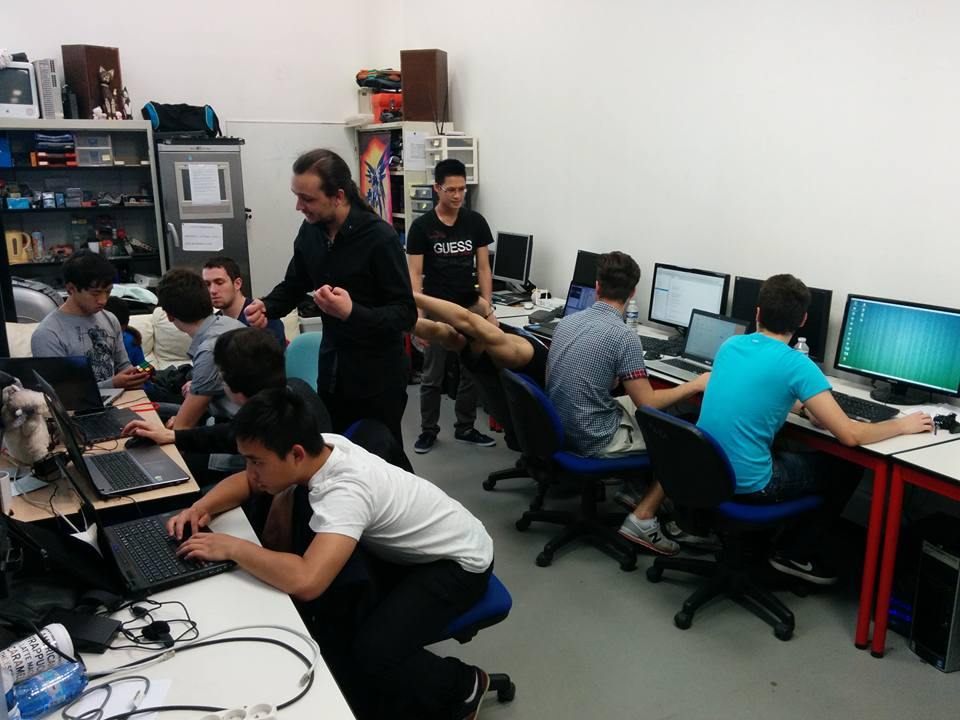
\includegraphics[width=90mm]{res/java-tutoring.jpg}
	\caption{Club*Nix aide en Java}
\end{figure}

\chapter{Membres}

\section{Effectifs}

% This is also an intro:
\paragraph{} Le Club*Nix a un totale de 56 inscrits. Et reçoit aussi des élevés extérieur au club pour les aidés temporairement lors des projets, ce qui nécessite une capacité variable.
\section{Membre actif}
\paragraph{} Le club est également un lieu de vie pour la plupart des membres
actifs du club, sur les membres inscrits, 15--20 personnes sont
présents en permanence dans la cellule reste souvent tard le soir que ce soit pour des projets 
associés à l'ESIEE ou internes au Club*Nix.

\part{Utilisation de la cellule}

\chapter{Inventaire}

\section{Machines}
\subsection{Ordinateur}
% Again, this is an intro:
\paragraph{} La cellule du Club*Nix nous permet d'avoir 6 ordinateurs sous
Linux, chacun ayant une distribution différente, à disposition pour tout
ESIEEens avec une assistance des membres du club qui se font un plaisir de
partager leurs connaissances.
\subsection{Serveur}
\paragraph{} Nous avons aussi à l'intérieur de la cellule 3 serveurs nous
permettant de desservir le site tu Club *Nix situé à l'adresse
\url{https://clubnix.fr}. Ils nous permettent aussi de stocker les fichiers et
dossiers des membres, ainsi que de leur fournir un compte complet avec
identifiant et mot de passe.



\section{Servisses mis à disposition}


\subsection{Canapé}
\paragraph{} Le Club*Nix est aussi un endroit de repos, et c'est pour cela que
nous avons un canapé au sein du club. Les membres peuvent se reposer afin
d'être plus concentrés en cours. Nous utilisons aussi un système de
climatisation pour rafraichir la cellule, sont utilisation serait compliquée
sans la fenêtre en façade.

% This however, is an intro:
\subsection{Frigo}
\paragraph{} Avoir une cellule nous permet également de posséder un frigo que
l'on remplit régulièrement de canettes ce qui nous permet de faire un peu
d'argent pour obtenir de nouvelles machines qui serviront, comme énoncé
précédemment, à aider les ESIEEens qui désirent développer leurs compétences
informatiques.

\subsection{Snacks}
\paragraph{} Le club mets aussi à disposition des snacks comme des barres de
Mars, des Kit Kats, etc\ldots, toujours à disposition des membres, ainsi qu'une
bouilloire et une cafetière et de la vaisselle pour permettre aux membres de
démarrer la journée de manière plus productive. Pour ceci nous possédons un
frigo qui est situé dans la cellule. Il nous serais difficile de stocker et
mettre a disposition ce service si nous manquions de place pour le frigo. 

\subsection{Casiers}
\paragraph{} Nous mettons aussi à disposition du matériel de stockage comme des
casiers réservés à des membres, ce qui permet par exemple, de venir à l'école
avec un sac moins pesant, ou d'avoir des documents à portée de main lorsque le
membre est dans la cellule.

\section{Matériel à disposition}
\subsection{Outils}
\paragraph{} Avec cela sont proposés aussi des outils mécaniques comme des
tournevis, pinces, cutters, mais aussi des outils électroniques comme quelques
composants, un fer à souder, et du matériel informatique comme des claviers,
souris, câbles Ethernet, câbles d'alimentation, USB, micro-USB, multiprises,
enceintes, switch, etc\ldots


\subsection{matériels scolaires}

\paragraph{} Du matériel scolaire et aussi disponible pour les membres comme
des dictionnaires d'anglais, des calculatrices, des règles et d'autres
instruments de mesures.

\subsection{Livres et Documentations}
\paragraph{} Il est aussi possible de lire dans la cellules des comics et
bandes-dessinées, des mangas, des livres/références/guides sur des sujet
principalement dans le domaine de l'informatique, comme le réseau, la sécurité,
la programmation.

\subsection{Tableaux}
\paragraph{} Afin que les membres puissent expliquer des idées, faire des
démonstrations, des schémas explicatifs. Le club a mit à disposition des grands
tableaux blancs. Ces tableaux servent aussi comme un moyen de communication.
Ceci renforce les échanges et facilites la compréhension entre les membres.


\subsection{Badges}
\paragraph{} La cellule actuelle possède un système de verrouillage
électronique avec badge. Plusieurs de nos membres on déjà fais l'empreint
nominatif de celui-ci.

\chapter{Membres}
\section{Consultation}
\paragraph{} Comme mentionné précédemment de la première partie, les membres du
Club *Nix viennent régulièrement dans la cellule et l'utilisent à fin de
travailler sur diverse matières, utilisent les ordinateurs du club pour
développer, apprendre, ou même aller sur internet ou regarder leurs mails.
\section{Projets}
\paragraph{} Ils utilisent la cellule également afin de stocker leurs projets
scolaires ou non, et travaillent aussi dessus à l'intérieur de la cellule.

\paragraph{} De nombreux membres se retrouvent le weekend pour finir et
continuer leurs projets. Certaine salles de cours étant fermées, le Club*Nix
permet de fournir lors des weekends des outils indispensable, tel qu'une
connexion au réseau de l'ESIEE pour continuer a utiliser ses outils.
\section{Echanges}
\paragraph{} Enfin et surtout, la cellule est utilisée comme lieu de vie pour
échanger et communiquer entre les membres, ce qui en fait pour les membres un
lieu privilégié pour travailler et discuter de sujets plus large que dans le
domaine de l'informatique.

\end{document}

% vim: spell : spelllang=fr
